\section{Introducción}

\begin{frame}{Introducción}
    \vspace{0.1cm}
    {\small
    Las simulaciones de \textit{n}-cuerpos modelan interacciones gravitacionales en sistemas estelares y planetarios, pero típicamente operan con \textbf{masas estáticas}, limitando su aplicabilidad en fenómenos dinámicos con variación de masas.
    }
    \vspace{0.2cm}
    \begin{figure}[H]
        \centering
        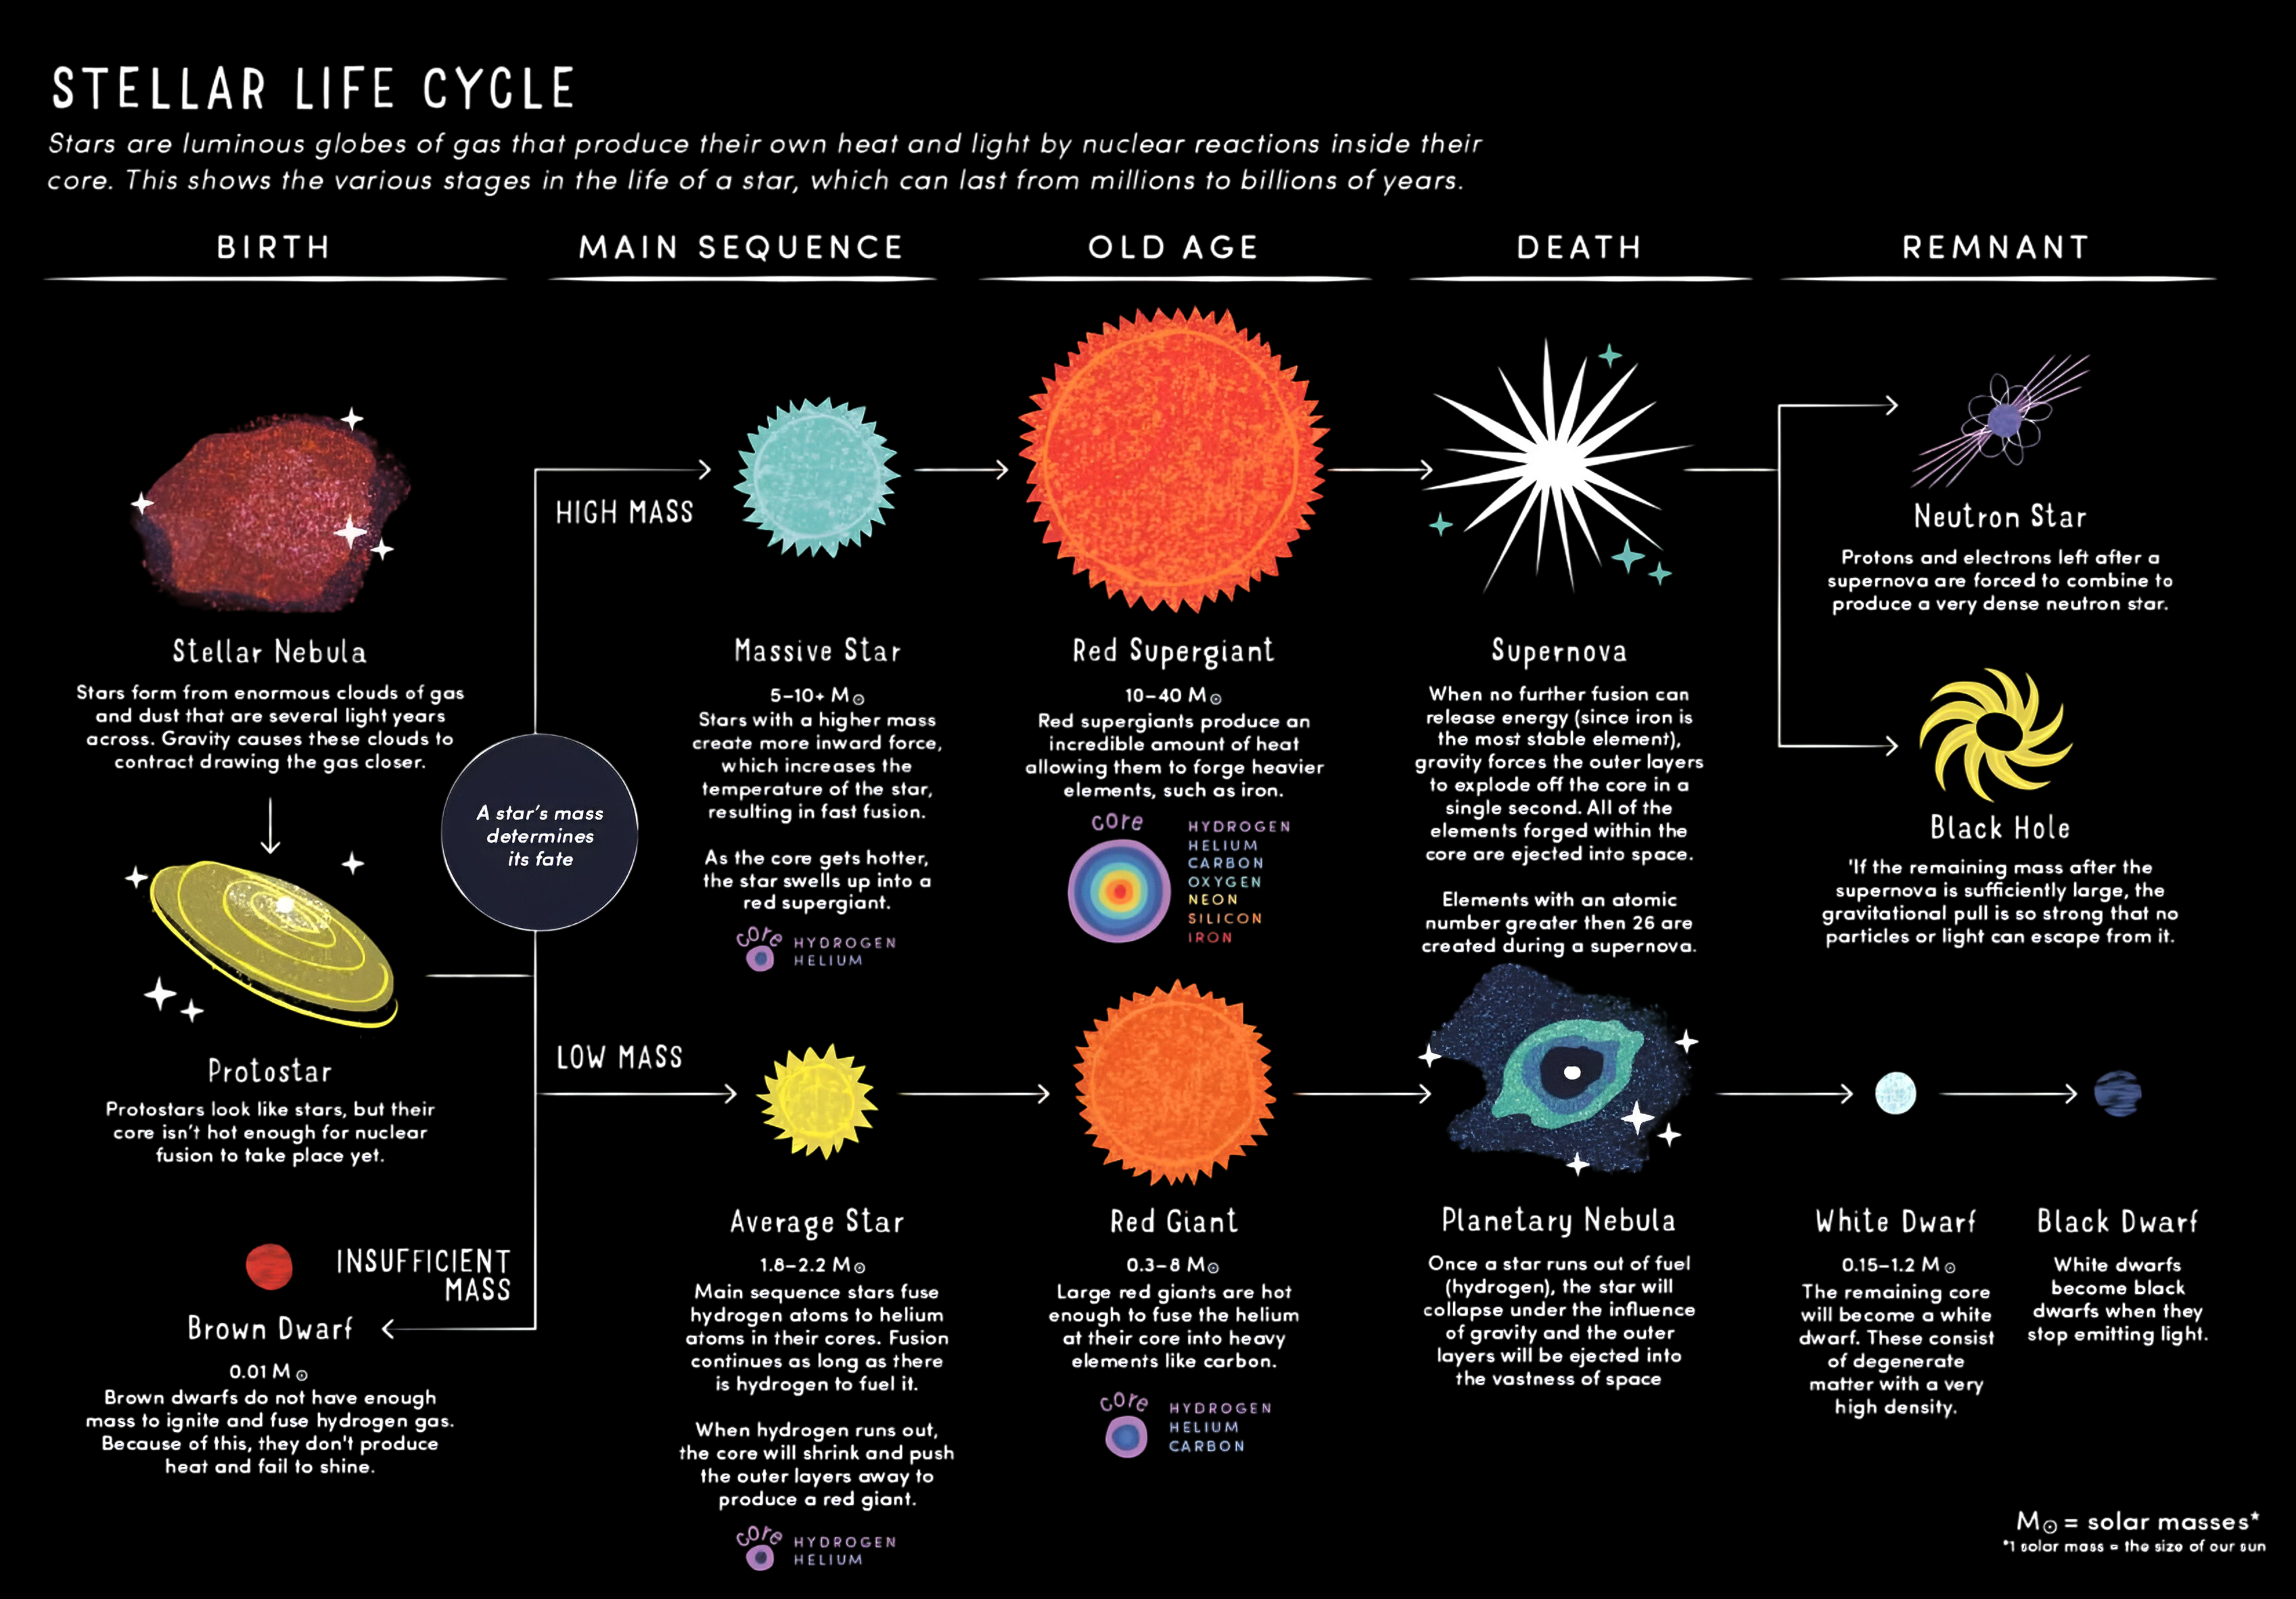
\includegraphics[width=0.75\textwidth, height=0.50\textheight, keepaspectratio]{img/introduccion/star-constellation-map.png}
        \vspace{-0.2cm}
        \caption{\tiny Ciclo de evolución estelar.~\textit{Fuente:}~\cite{smartyprints_constellation_poster_2025}}%
    \end{figure}
\end{frame}

\begin{frame}{Planteamiento del Problema}
    \vspace{0.1cm}
    \begin{columns}
        \begin{column}{0.55\textwidth}
            {\small
            \textbf{Limitación actual:}
            \begin{itemize}
                \item Masas invariables en simulaciones tradicionales
                \item Afecta estabilidad en fenómenos dinámicos
                \item Reduce aplicabilidad en sistemas de $n$-cuerpos.
            \end{itemize}
            \vspace{0.2cm}
            \textbf{Métrica de estabilidad:}\\
            Exponente de Lyapunov para cuantificar comportamiento caótico.
            }
        \end{column}
        \begin{column}{0.45\textwidth}
            \centering
            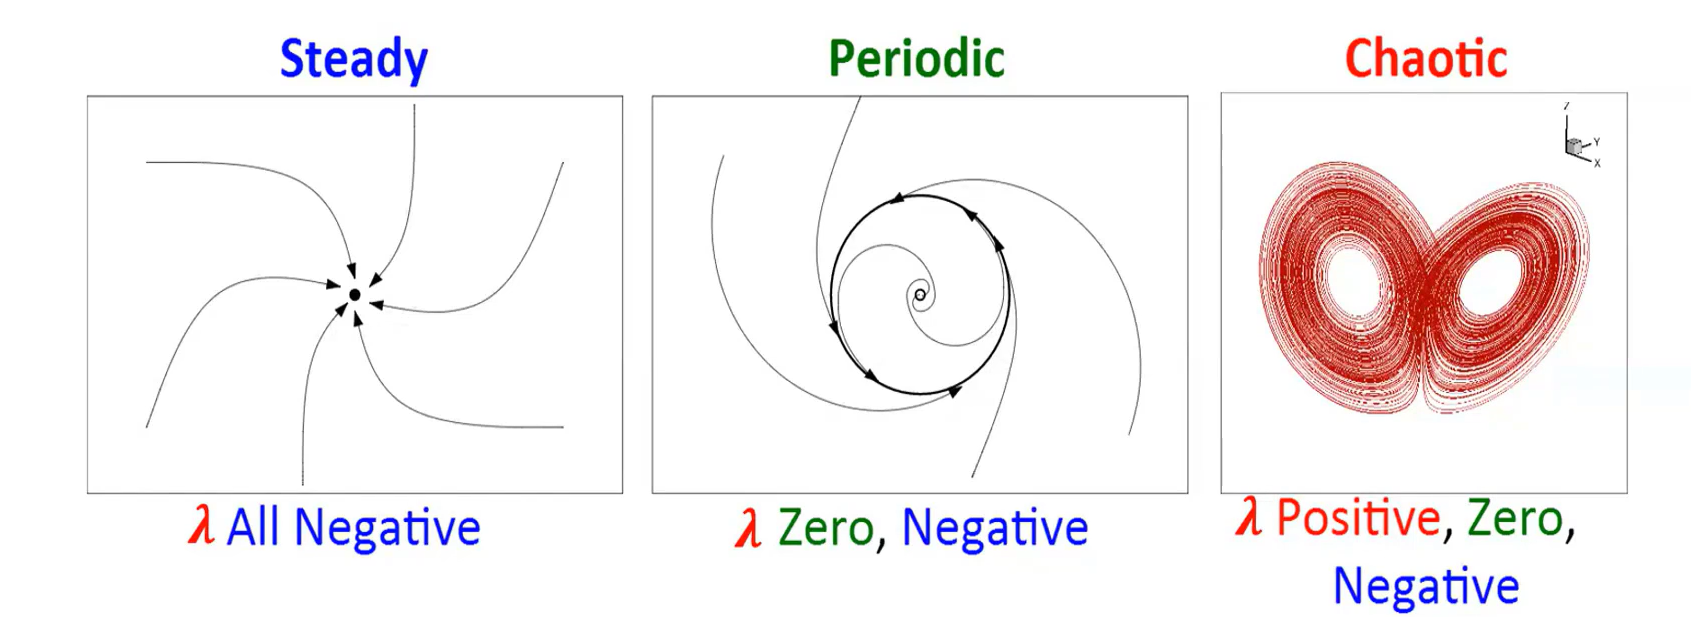
\includegraphics[width=\textwidth, height=0.55\textheight, keepaspectratio]{img/introduccion/lyapunov.png}
            \vspace{-0.2cm}
            {\tiny Comportamientos según exponente de Lyapunov.~\cite{wang_numerical_methods_2014}}
        \end{column}
    \end{columns}
\end{frame}

\begin{frame}{Propuesta de Solución}
    \vspace{0.1cm}
    \begin{columns}
        \begin{column}{0.40\textwidth}
            {\small
            Modelo de optimización con:
            \begin{itemize}
                \item \textbf{Modificación dinámica de masas} en tiempo de ejecución
                \item \textbf{Algoritmos genéticos} para ajuste paramétrico
                \item \textbf{Mejora de estabilidad} mediante optimización de Lyapunov
            \end{itemize}
            }
        \end{column}
        \begin{column}{0.60\textwidth}
            \centering
            \fbox{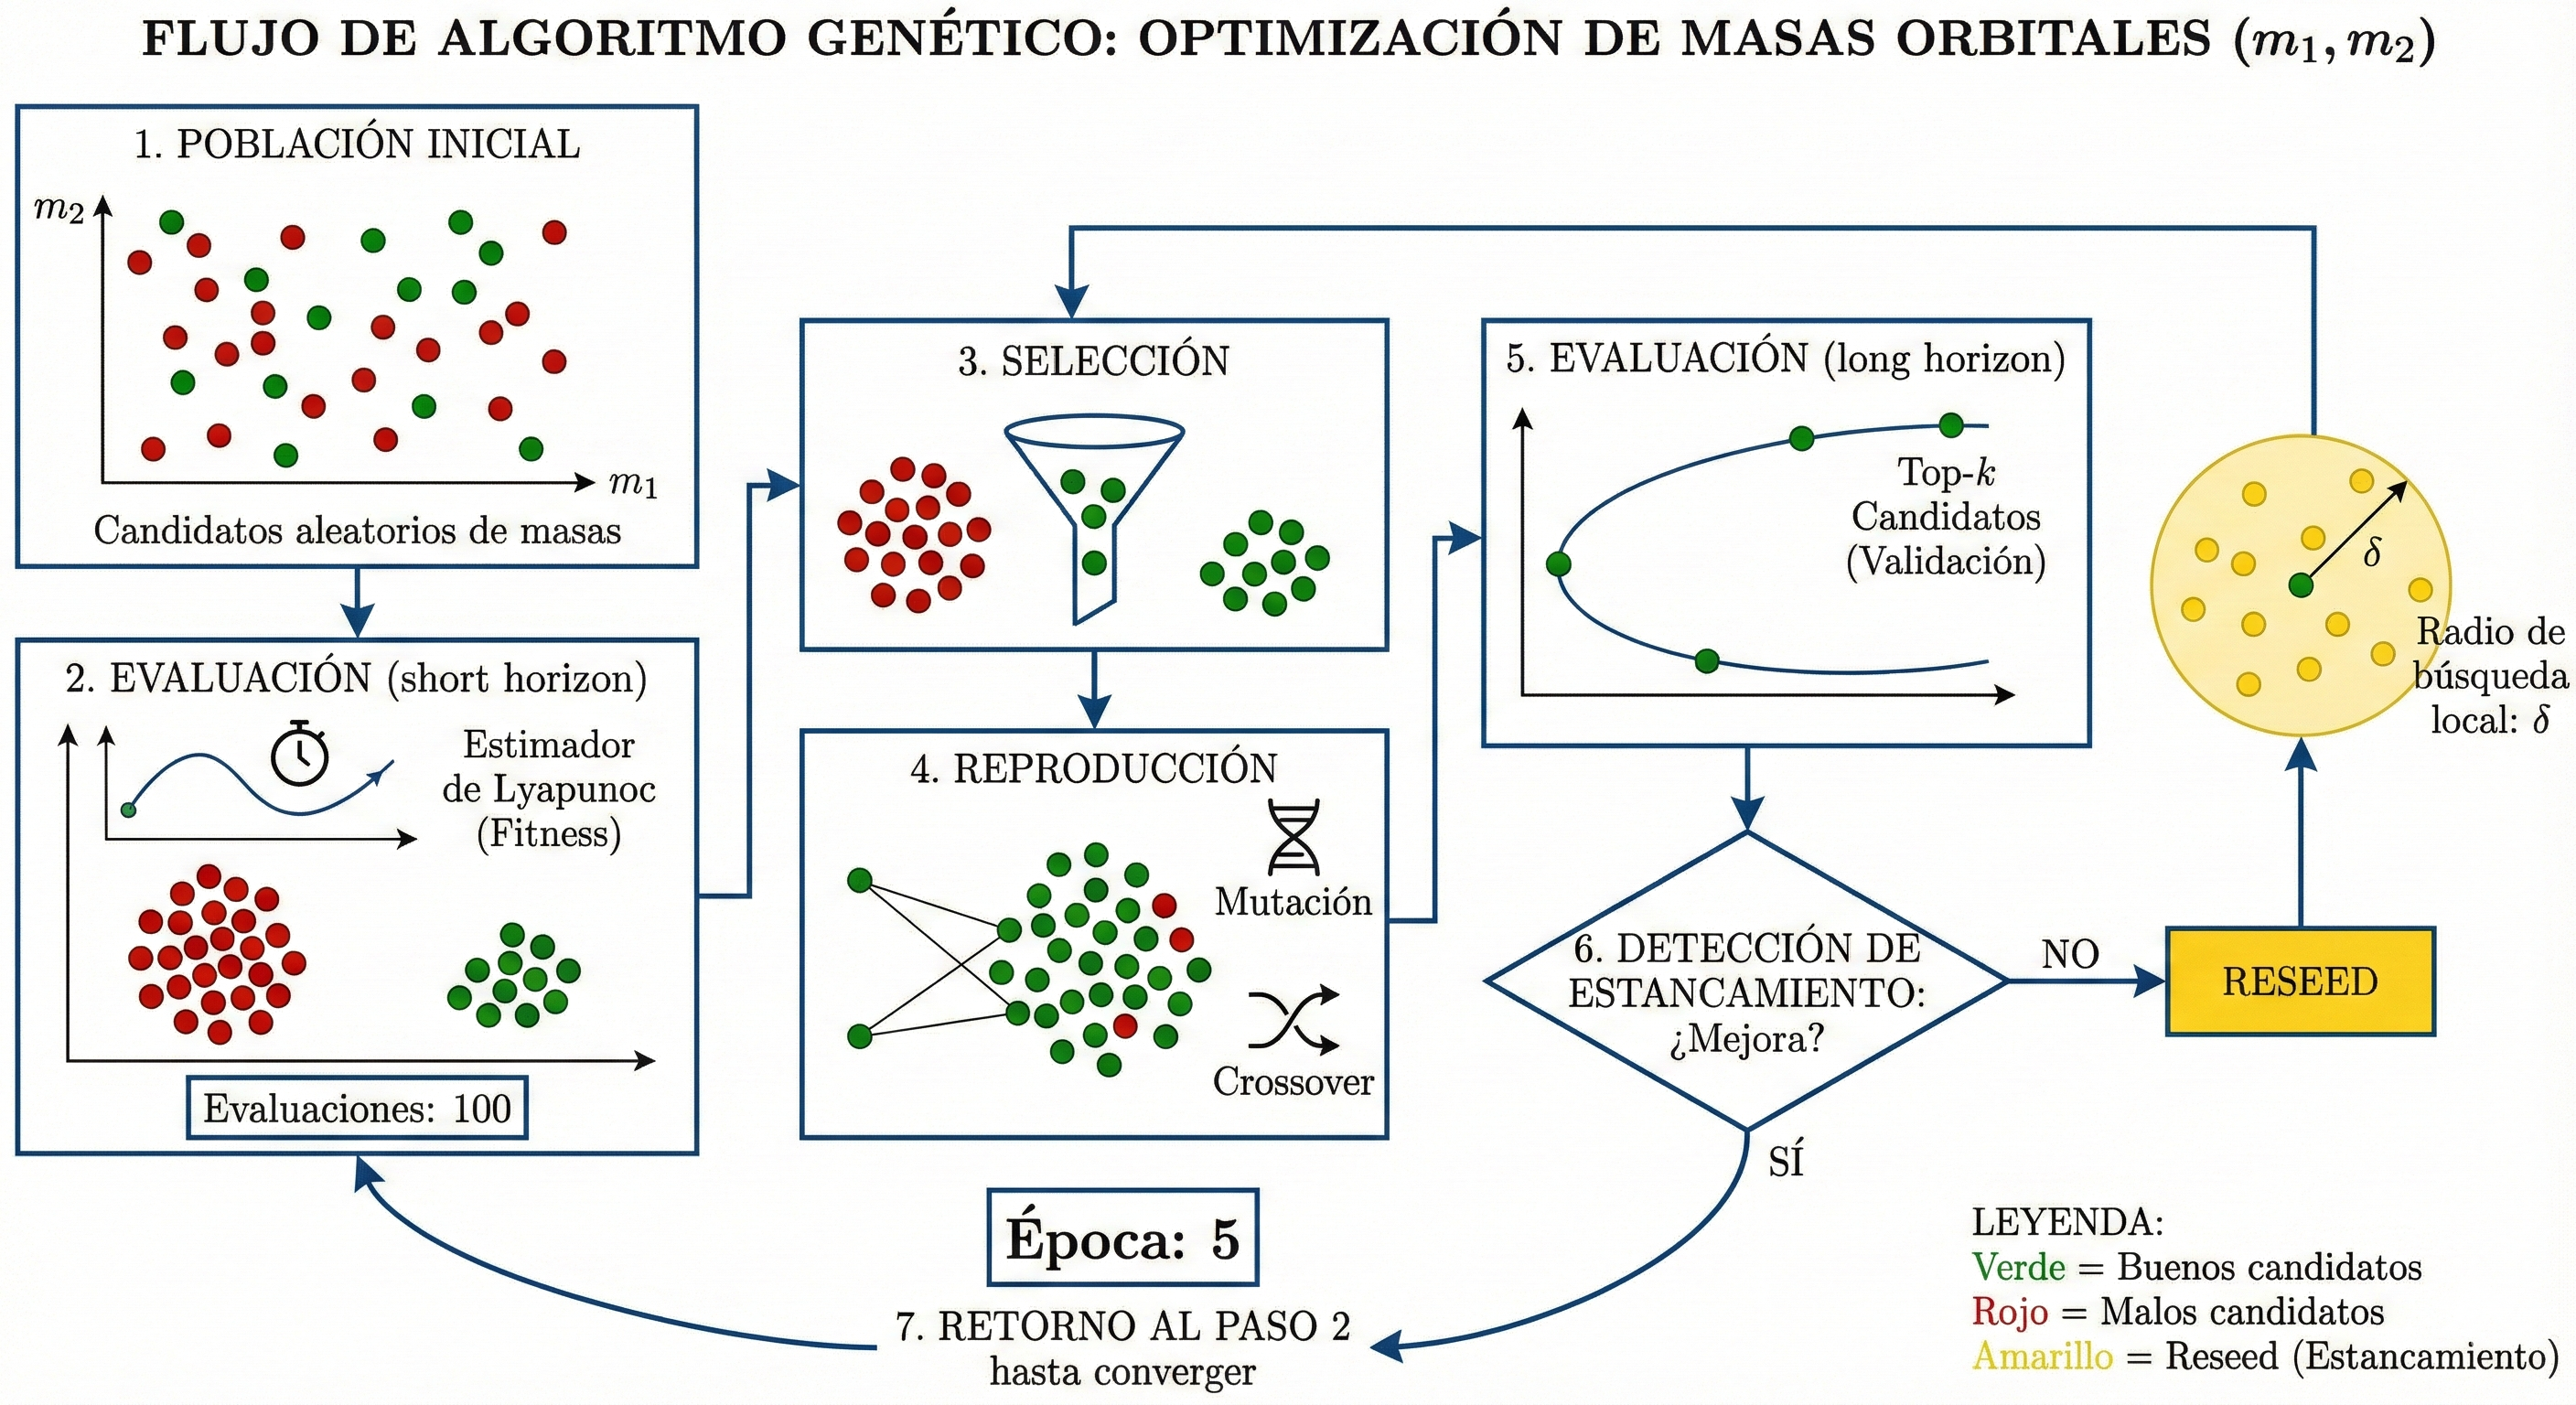
\includegraphics[width=0.95\textwidth, height=0.65\textheight, keepaspectratio]{img/introduccion/AlgoritmoGenetico.png}}
            \vspace{-0.2cm}
            {\tiny Aplicación de algoritmo genético.~\textit{Autoría Propia}}
        \end{column}
    \end{columns}
\end{frame}

\begin{frame}{Hipótesis}
    \vspace{0.1cm}
    {\small
    Modificar dinámicamente la masa en simulaciones de dos cuerpos, mediante algoritmos bioinspirados y métodos eficientes de cálculo gravitacional, permitirá alcanzar una \textbf{estabilidad local superior} (menor exponente de Lyapunov) frente a simuladores tradicionales con parámetros estáticos.
    }
    \vspace{0.2cm}
    \begin{figure}[H]
        \centering
        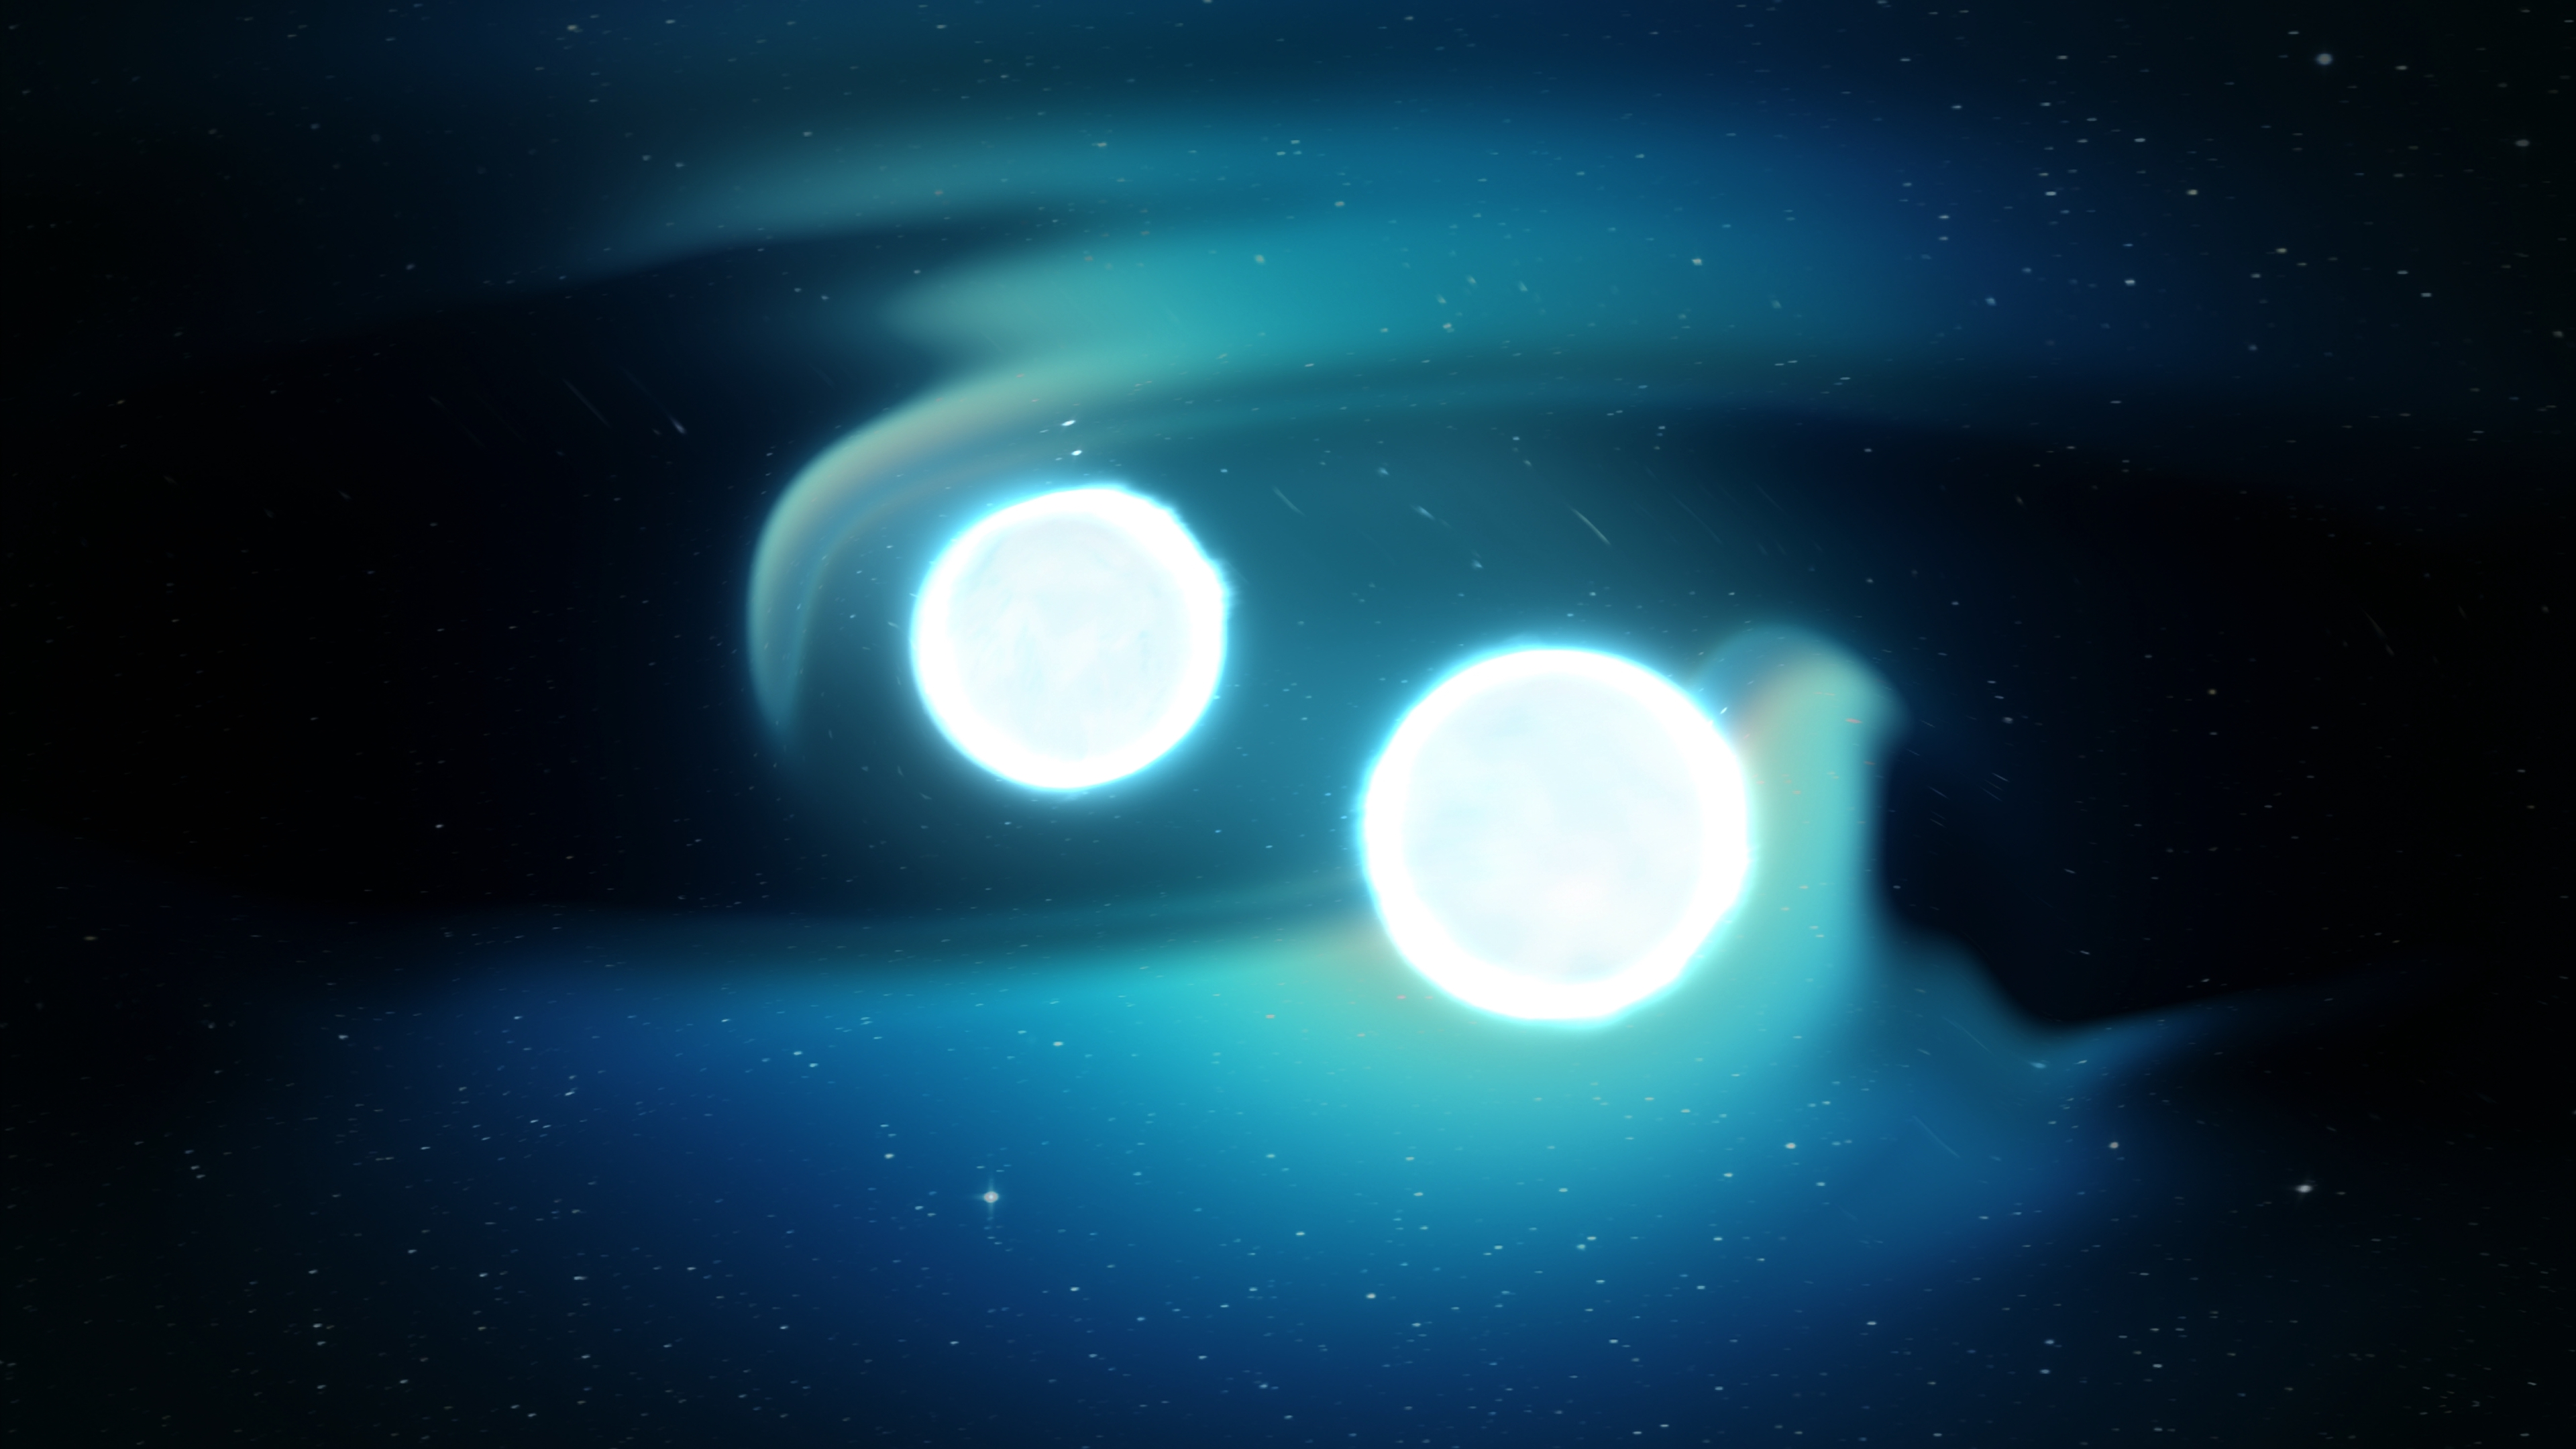
\includegraphics[width=0.7\textwidth, height=0.50\textheight, keepaspectratio]{img/introduccion/Neutron_Star_Merger_Still_1.jpg}
        \vspace{-0.2cm}
        \caption{\tiny Colisión de estrellas de neutrones (simulación).~\cite{nasa_star_collision_2018}}%
    \end{figure}
\end{frame}

%\begin{frame}{Objetivo General}
%    \vspace{0.2cm}
%    \begin{minipage}[c]{0.6\textwidth}
%        {\small
%        Desarrollar un modelo de optimización para simulación de 2-3 cuerpos que permita la \textbf{modificación dinámica de masas}, mejorando la estabilidad local mediante reducción del exponente de Lyapunov.
%        }
%    \end{minipage}
%    \hfill
%    \begin{minipage}[c]{0.35\textwidth}
%        \centering
%        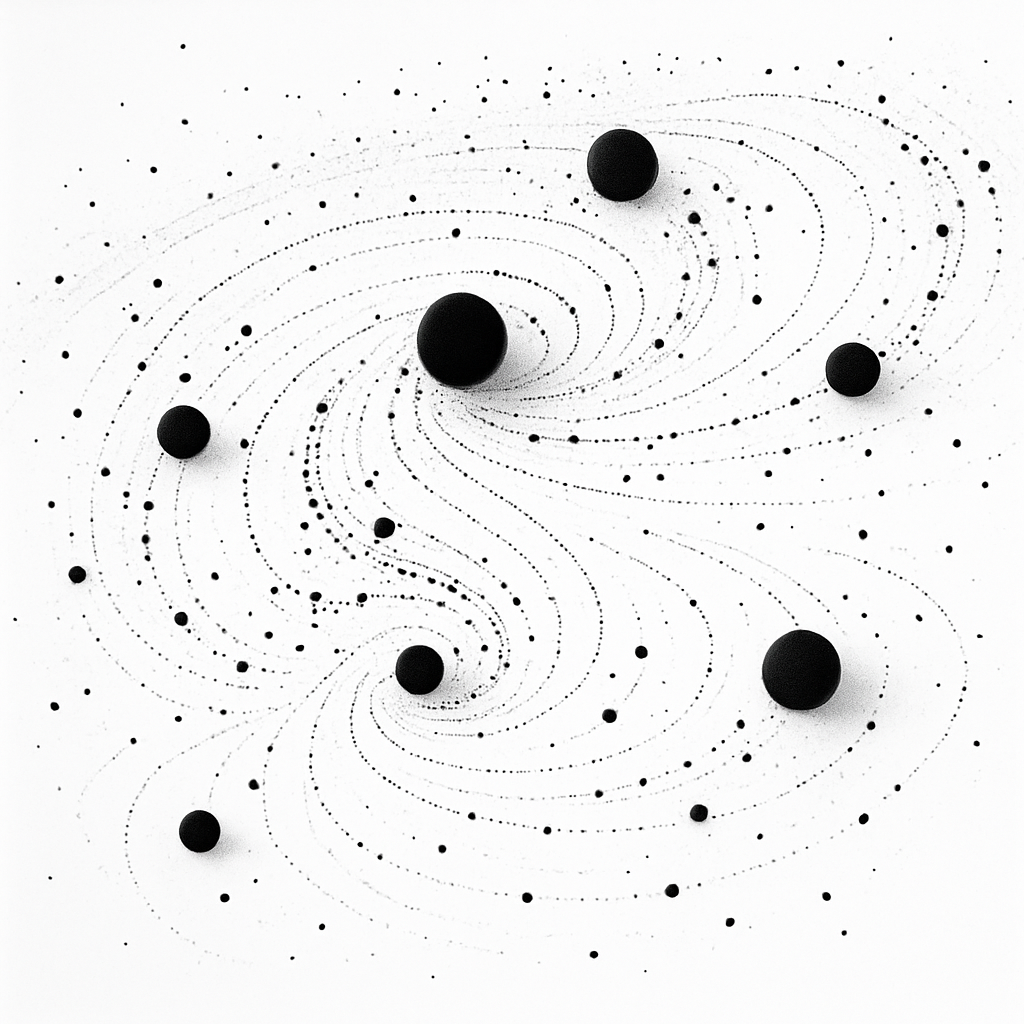
\includegraphics[width=\textwidth, height=0.45\textheight, keepaspectratio]{img/introduccion/n-body-representation.png}
%        \vspace{-0.2cm}
%        {\tiny Sistema de \textit{n}-cuerpos.~\textit{Autoría Propia}}
%    \end{minipage}
%\end{frame}
%
%\begin{frame}{Objetivos Específicos}
%    \vspace{0.1cm}
%    {\small
%    \begin{itemize}
%        \item \textbf{Simulación}: Integración numérica usando REBOUND (IAS15/WHFAST).
%        \item \textbf{Optimización}: Algoritmo genético para ajuste dinámico de masas.
%        \item \textbf{Estabilidad}: Cálculo del exponente de Lyapunov como métrica de caos.
%        \item \textbf{Visualización}: Representación 2D/3D de trayectorias.
%        \item \textbf{Instrumentación}: Telemetría para análisis de rendimiento.
%    \end{itemize}
%    }
%\end{frame}
%